% !TEX root = morphkasten.tex

\section{Microcontroller}


%##############
\subsection{Freedom-Board}

Grafik

\begin{table}[h]
\begin{tabular}{p{0.5\textwidth} | p{0.5\textwidth}}


 \textbf{Vorteile} & \textbf{Nachteile} \\ \hline
	 
\begin{itemize}
\item Vorteil 1
\item Vorteil 2
\item Vorteil 3
\item ...
\end{itemize}

 
 &
 
\begin{itemize}
\item Nachteil 1
\item Nachteil 2
\item Nachteil 3
\item ...
\end{itemize}

\end{tabular}
\end{table}

\begin{table}[h]
\begin{tabular}{p{0.5\textwidth}p{0.5\textwidth}}


 \textbf{Risiken} & \\ \hline
	 
\begin{itemize}
\item Risiko 1
\item Risiko 2
\end{itemize}
&
\begin{itemize}
\item Risiko 3
\item ...
\end{itemize}

 
\end{tabular}
\end{table}

\pagebreak


%##############
\subsection{Thinkerforge}
\begin{figure}[h]
	\centering
	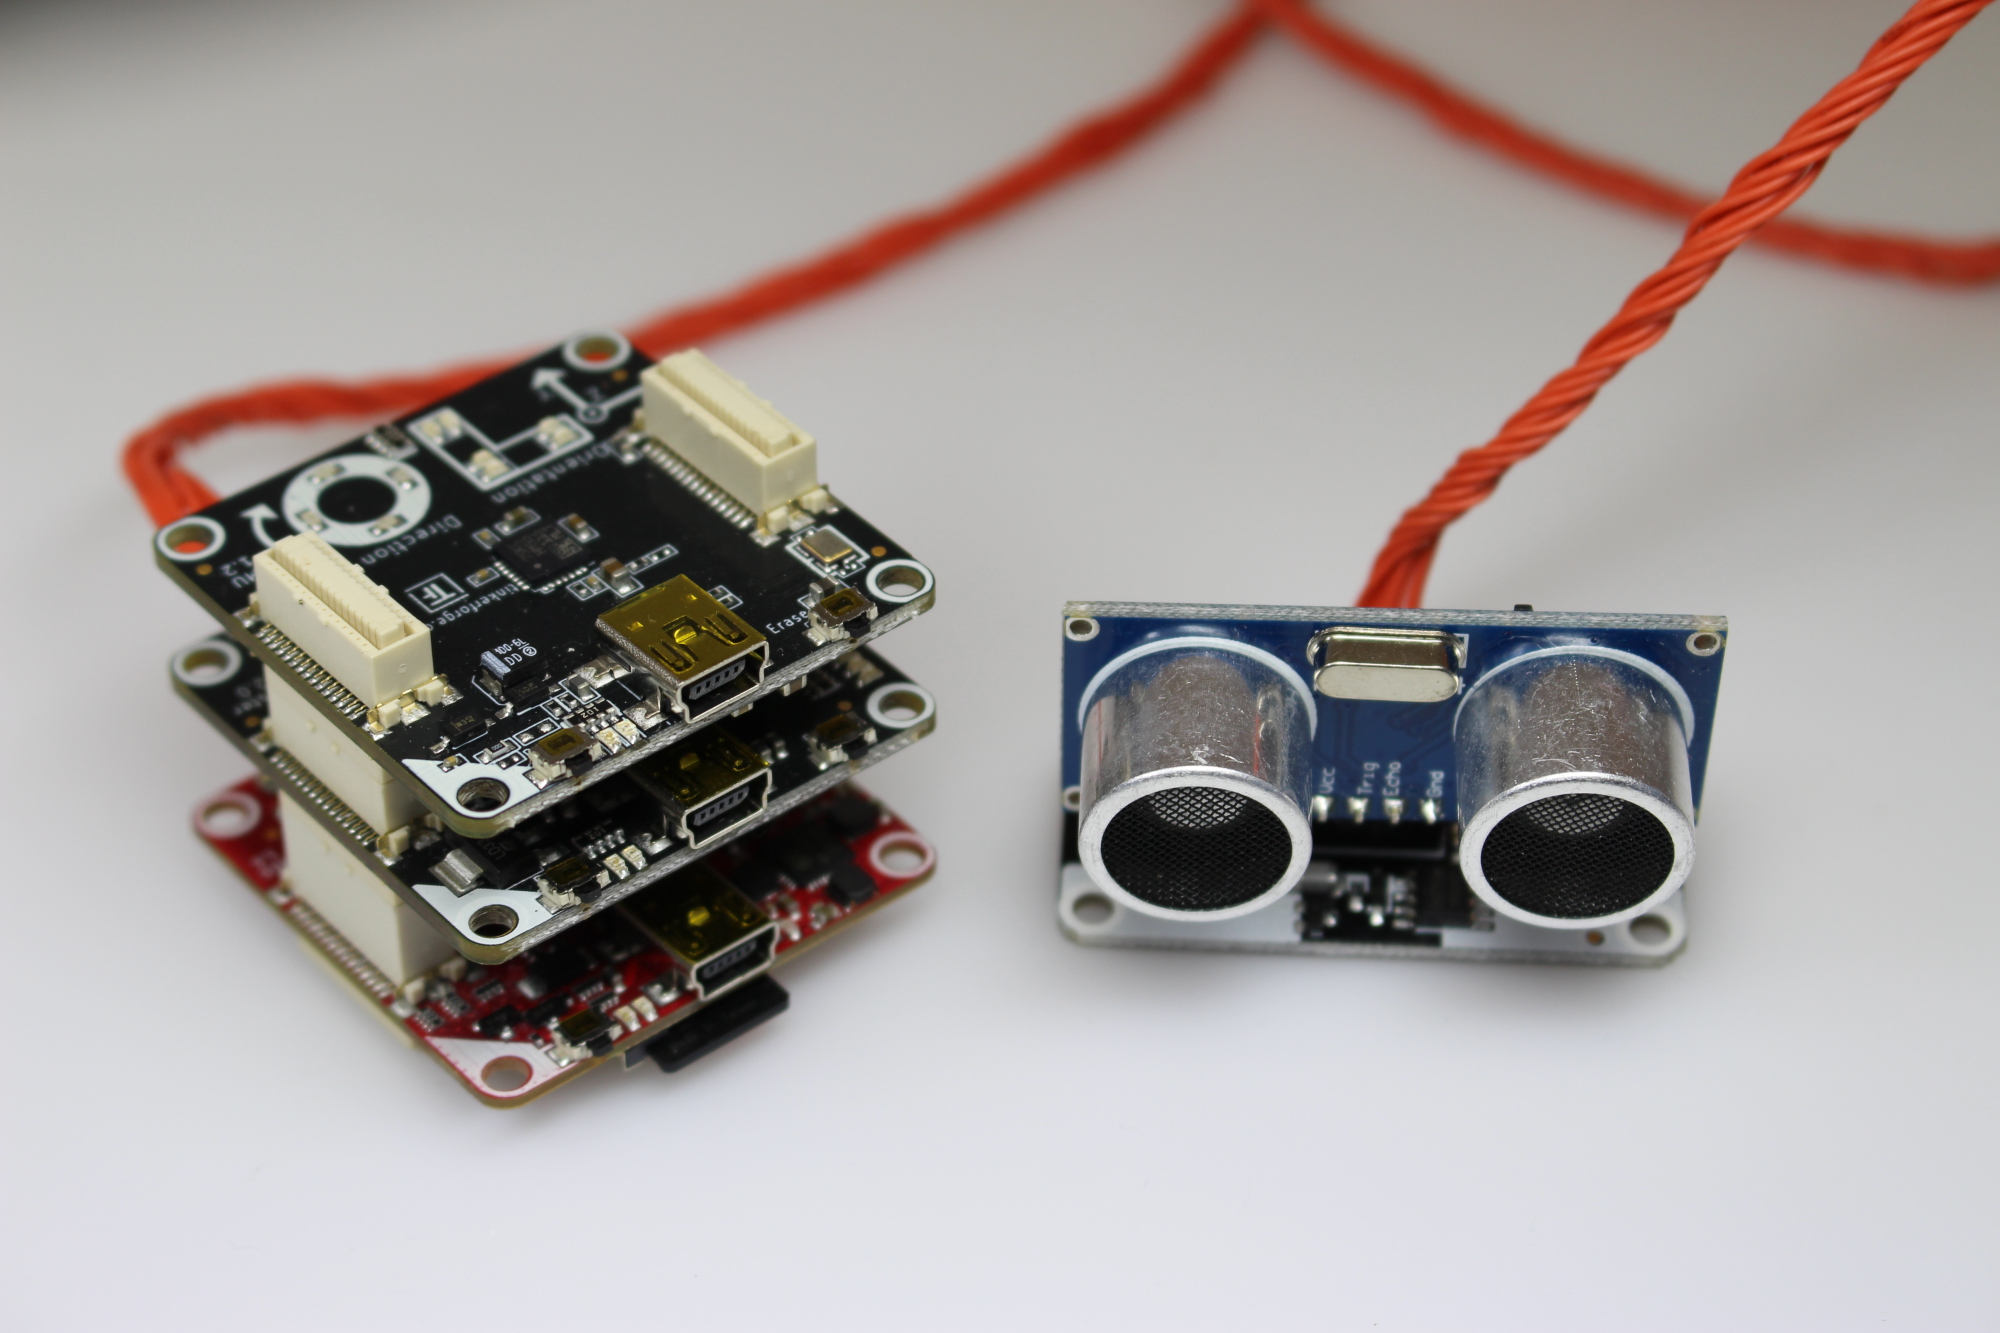
\includegraphics[width=0.5\textwidth]{fig/Tinkerforge.png}
	\caption{Beispielhaftes Tinkerforge System (Bricks mit Ultraschallmodul)}
\end{figure}

\begin{table}[h]
\begin{tabular}{p{0.5\textwidth} | p{0.5\textwidth}}


\textbf{Vorteile} & \textbf{Nachteile} \\ \hline
	 
\begin{itemize}
\item Einfache und modulare Schnittstelle zum Boardcomputer
\item Einfach erweiterbar mit zusätzlichen Modulen (z.B Sensoren)
\item Viele benötigte Module Vorhanden: Schrittmotoren, Distanzsensoren, Liniensensoren und Farbsensoren
\end{itemize}
 &
\begin{itemize}
\item Grosser Aufwand für eigene Module(Abhängigkeit zu Tinkerforge)
\end{itemize}
\end{tabular}
\end{table}


\begin{table}[h]
\begin{tabular}{p{0.5\textwidth}p{0.5\textwidth}}


 \textbf{Risiken} & \\ \hline
	 
\begin{itemize}
\item Risiko 1
\item Risiko 2
\end{itemize}
&
\begin{itemize}
\item Risiko 3
\item ...
\end{itemize}

 
\end{tabular}
\end{table}

\pagebreak

%##############
\subsection{HCS08}
Grafik

\begin{table}[h]
\begin{tabular}{p{0.5\textwidth} | p{0.5\textwidth}}


 \textbf{Vorteile} & \textbf{Nachteile} \\ \hline
	 
\begin{itemize}
\item Vorteil 1
\item Vorteil 2
\item Vorteil 3
\item ...
\end{itemize}

 
 &
 
\begin{itemize}
\item Nachteil 1
\item Nachteil 2
\item Nachteil 3
\item ...
\end{itemize}

\end{tabular}
\end{table}

\begin{table}[h]
\begin{tabular}{p{0.5\textwidth}p{0.5\textwidth}}


 \textbf{Risiken} & \\ \hline
	 
\begin{itemize}
\item Risiko 1
\item Risiko 2
\end{itemize}
&
\begin{itemize}
\item Risiko 3
\item ...
\end{itemize}

 
\end{tabular}
\end{table}

\pagebreak